\documentclass[10pt]{article}
\usepackage[a4paper, margin=.9in]{geometry}
% \usepackage{xeCJK}
% \setCJKmainfont{Microsoft YaHei} 
\newcommand{\DOUBLECOL}{}	% turns this on for double column
\newlength{\subfigureheight}
\newlength{\figurewidth}
\ifdefined\DOUBLECOL
\setlength{\subfigureheight}{2.45in}
\setlength{\figurewidth}{3.5in}
\else
\setlength{\subfigureheight}{2.35in}
\setlength{\figurewidth}{6.5in}
\fi
\usepackage{amsfonts,amsmath,amssymb,bm,cancel,color,comment,epsfig,enumerate,empheq,floatrow,hyperref,mathdots,mathrsfs}
\usepackage{placeins}%\usepackage{algorithmic}
\usepackage[vlined,ruled,linesnumbered]{algorithm2e}
\SetKwInput{KwInput}{Input}                % Set the Input
\SetKwInput{KwOutput}{Output}              % set the Output
\SetKwRepeat{Do}{do}{until}%
\usepackage{graphicx}
%\usepackage{amsthm}
\usepackage[super]{nth}
\usepackage[noadjust]{cite}
\usepackage{subcaption}
\usepackage{tabularx}
\usepackage{tabularray}		% make thing horizontal lines in tabular
\UseTblrLibrary{booktabs}	% make thing horizontal lines in tabular

\usepackage{listings}
\usepackage{xcolor}

% --- MATLAB code style ---
\lstdefinelanguage{Matlab}{
  morekeywords={break,case,catch,continue,else,elseif,end,for,function,
    global,if,otherwise,persistent,return,switch,try,while},
  sensitive=true,
  morecomment=[l]\%,
  morestring=[m]',
}
\lstset{
  language=Matlab,
  basicstyle=\ttfamily\small,
  keywordstyle=\color{blue}\bfseries,
  commentstyle=\color{gray},
  stringstyle=\color{red!70!black},
  numbers=left,
  numberstyle=\tiny,
  stepnumber=1,
  numbersep=5pt,
  frame=single,
  breaklines=true,
  showstringspaces=false,
  columns=fullflexible
}


% --- TikZ setup ---
\usepackage{tikz}
\usetikzlibrary{arrows.meta,positioning}

\tikzset{
  >=Latex,
  block/.style={
    draw,
    rounded corners,
    minimum height=1.0cm,
    minimum width=2.6cm,
    align=center
  },
  io/.style={font=\small}
}

\hypersetup{
	colorlinks=true,
	linkcolor=red,
	citecolor=green,
	filecolor=magenta,
	urlcolor=blue
}


\newenvironment{Ualgorithm}[1][htpb]{\def\@algocf@post@ruled{\kern\interspacealgoruled\hrule  height\algoheightrule\kern3pt\relax}%
\def\@algocf@capt@ruled{under}
\begin{algorithm}[#1]}
{\end{algorithm}}

\setcounter{MaxMatrixCols}{30}
\DeclareSymbolFont{grb}{OML}{cmm}{b}{it}
\DeclareMathSymbol{\zetab}{\mathord}{grb}{"10}
\DeclareMathSymbol{\etab}{\mathord}{grb}{"11}
\DeclareMathSymbol{\thetab}{\mathord}{grb}{"12}
\DeclareMathSymbol{\kappab}{\mathord}{grb}{"14}
\DeclareMathSymbol{\lambdab}{\mathord}{grb}{"15}
\DeclareMathSymbol{\mub}{\mathord}{grb}{"16}
\DeclareMathSymbol{\nub}{\mathord}{grb}{"17}
\DeclareMathSymbol{\rhob}{\mathord}{grb}{"1A}
\DeclareMathSymbol{\sigmab}{\mathord}{grb}{"1B}
\DeclareMathSymbol{\taub}{\mathord}{grb}{"1C}
\DeclareMathSymbol{\phib}{\mathord}{grb}{"1E}
\DeclareMathSymbol{\psib}{\mathord}{grb}{"20}
\DeclareMathSymbol{\omegab}{\mathord}{grb}{"21}
\DeclareMathSymbol{\epsilonb}{\mathord}{grb}{"22}
\DeclareMathSymbol{\varphib}{\mathord}{grb}{"27}
\input{Symbol_Shortcut.tex}

\newtheorem{theorem}{\bf Theorem}		% by Victor
\newtheorem{corollary}{\bf Corollary}	% by Victor
\newtheorem{definition}{\bf Definition}	% by Victor


\makeatletter
\def\ifundefined{\@ifundefined}
\makeatother

\setlength{\parskip}{0ex}

\newcommand\fH[1]{\sbox0{#1}\dimen0=\ht0 \advance\dimen0 -1ex
  \sbox2{\'{}}\sbox2{\raise\dimen0\box2}%
  {\ooalign{\hidewidth\kern.1em\copy2\kern-.5\wd2\box2\hidewidth\cr\box0\crcr}}}

\title{\vspace{-0.2em} \huge LAB3 Report}
\author{Pin-Jing, Li (111511015 \it{ouo.ee11@nycu.edu.tw})\\ 
Ching-Kai, Huang (111511151 \it{kevin.ee11@nycu.edu.tw})\\ 
Duan-Kai, Hu (112511015 \it{huduankai@gmail.com})}




\begin{document}
\maketitle

\section{Data Pre-Processing}



\section{Experiment I: Car movement}
\subsection{Calibration}
This section talks about the calibration on the accelleration detector of the IMU. We make use of the gravity $1g = 16384$ as our reference.
The work flow is as follow,
\begin{itemize}
  \item[1] Face the target direction upward and collect the signal. 
  \item[2] Obtain the mean of the target direction in raw unit with \lstinline|meas_mean = mean(target_axis)|
  \item[3] Obtain the desired correction term \lstinline|b_axis  = a_exp - meas_mean| with  \lstinline|a_exp = 16384|
\end{itemize}

The following set of figures shows the signal before and after the calibration.

\begin{figure}[!h]
	\centering
	\subcaptionbox{x positive
		\label{fig:calib_xp}}{
		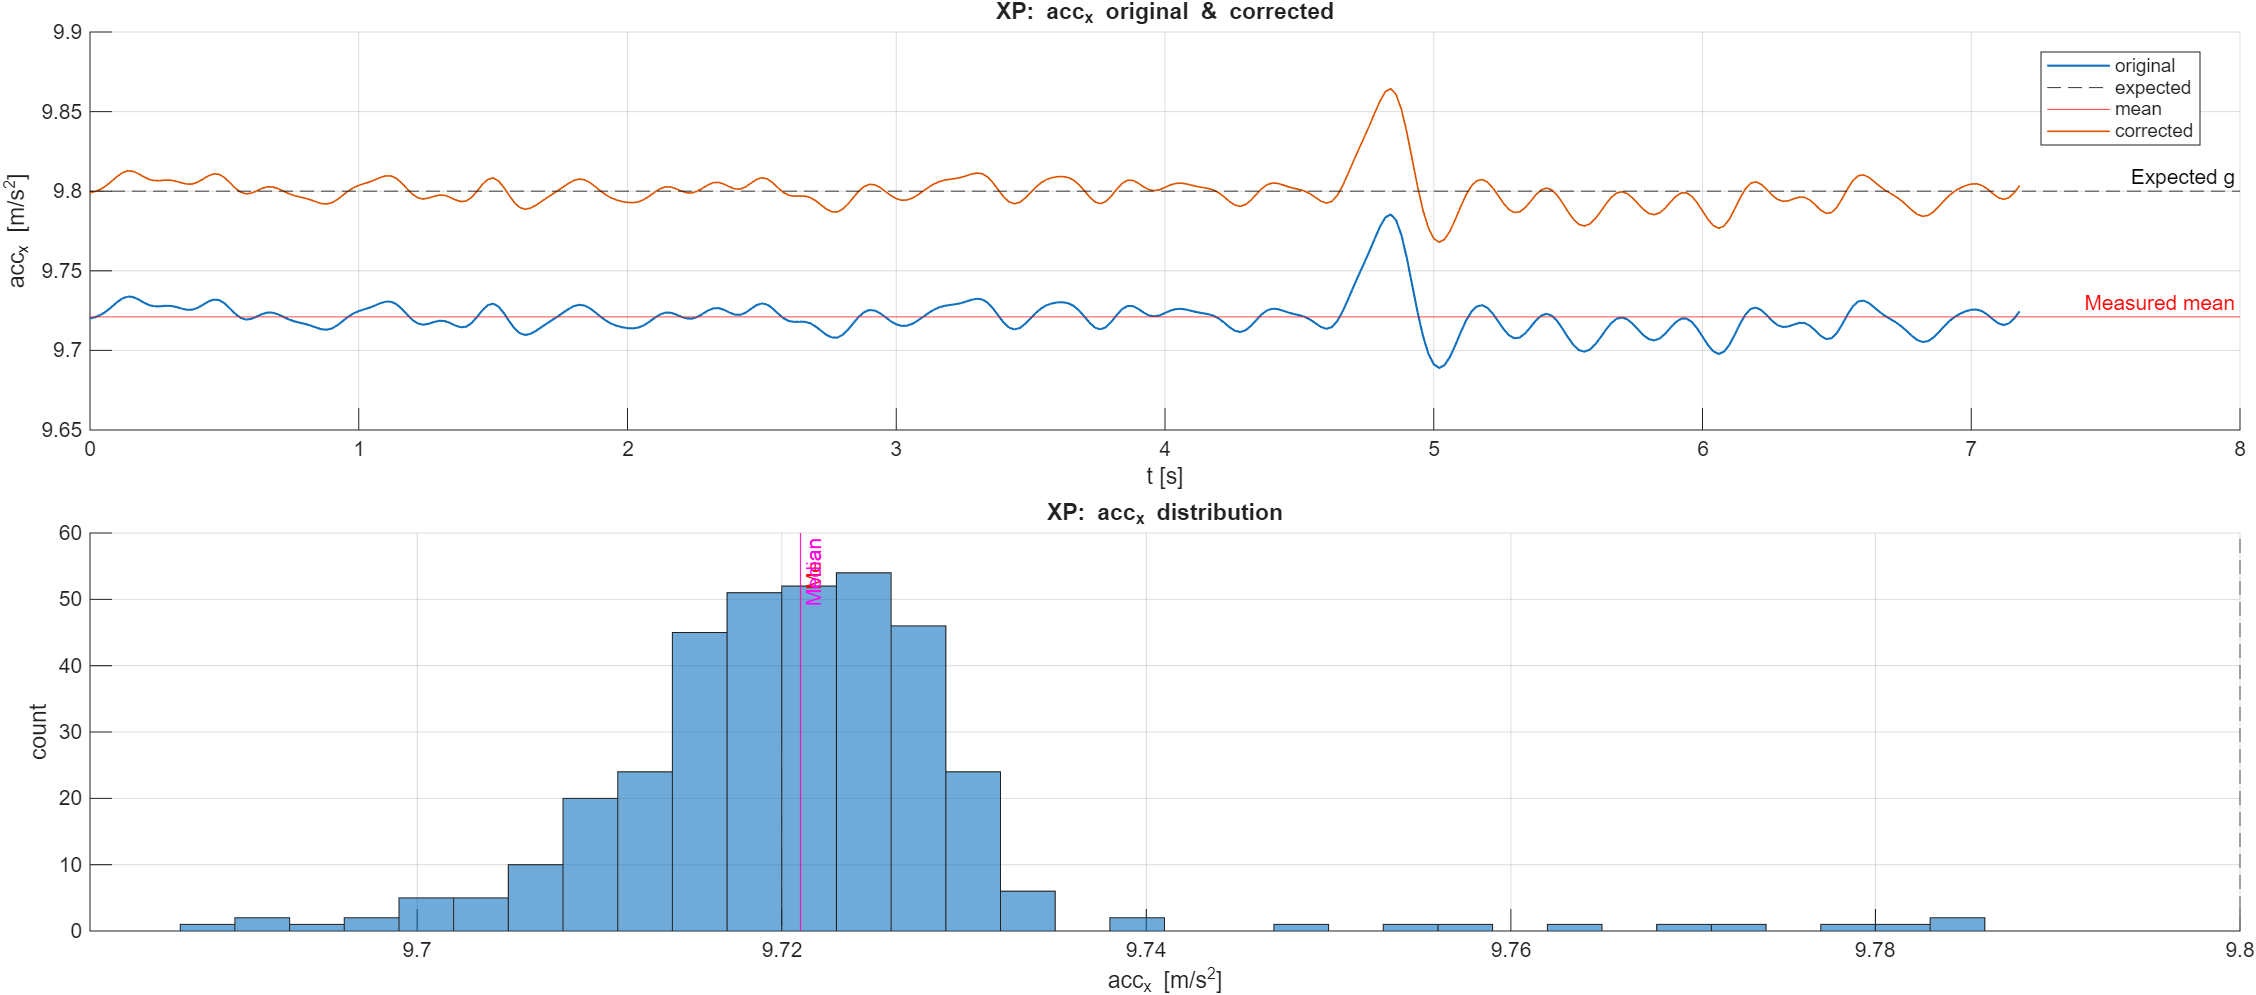
\includegraphics[width=0.3\columnwidth]{fig/Gravity check XP - acc_x.png}}
	\subcaptionbox{y positive
		\label{fig:calib_yp}}{
		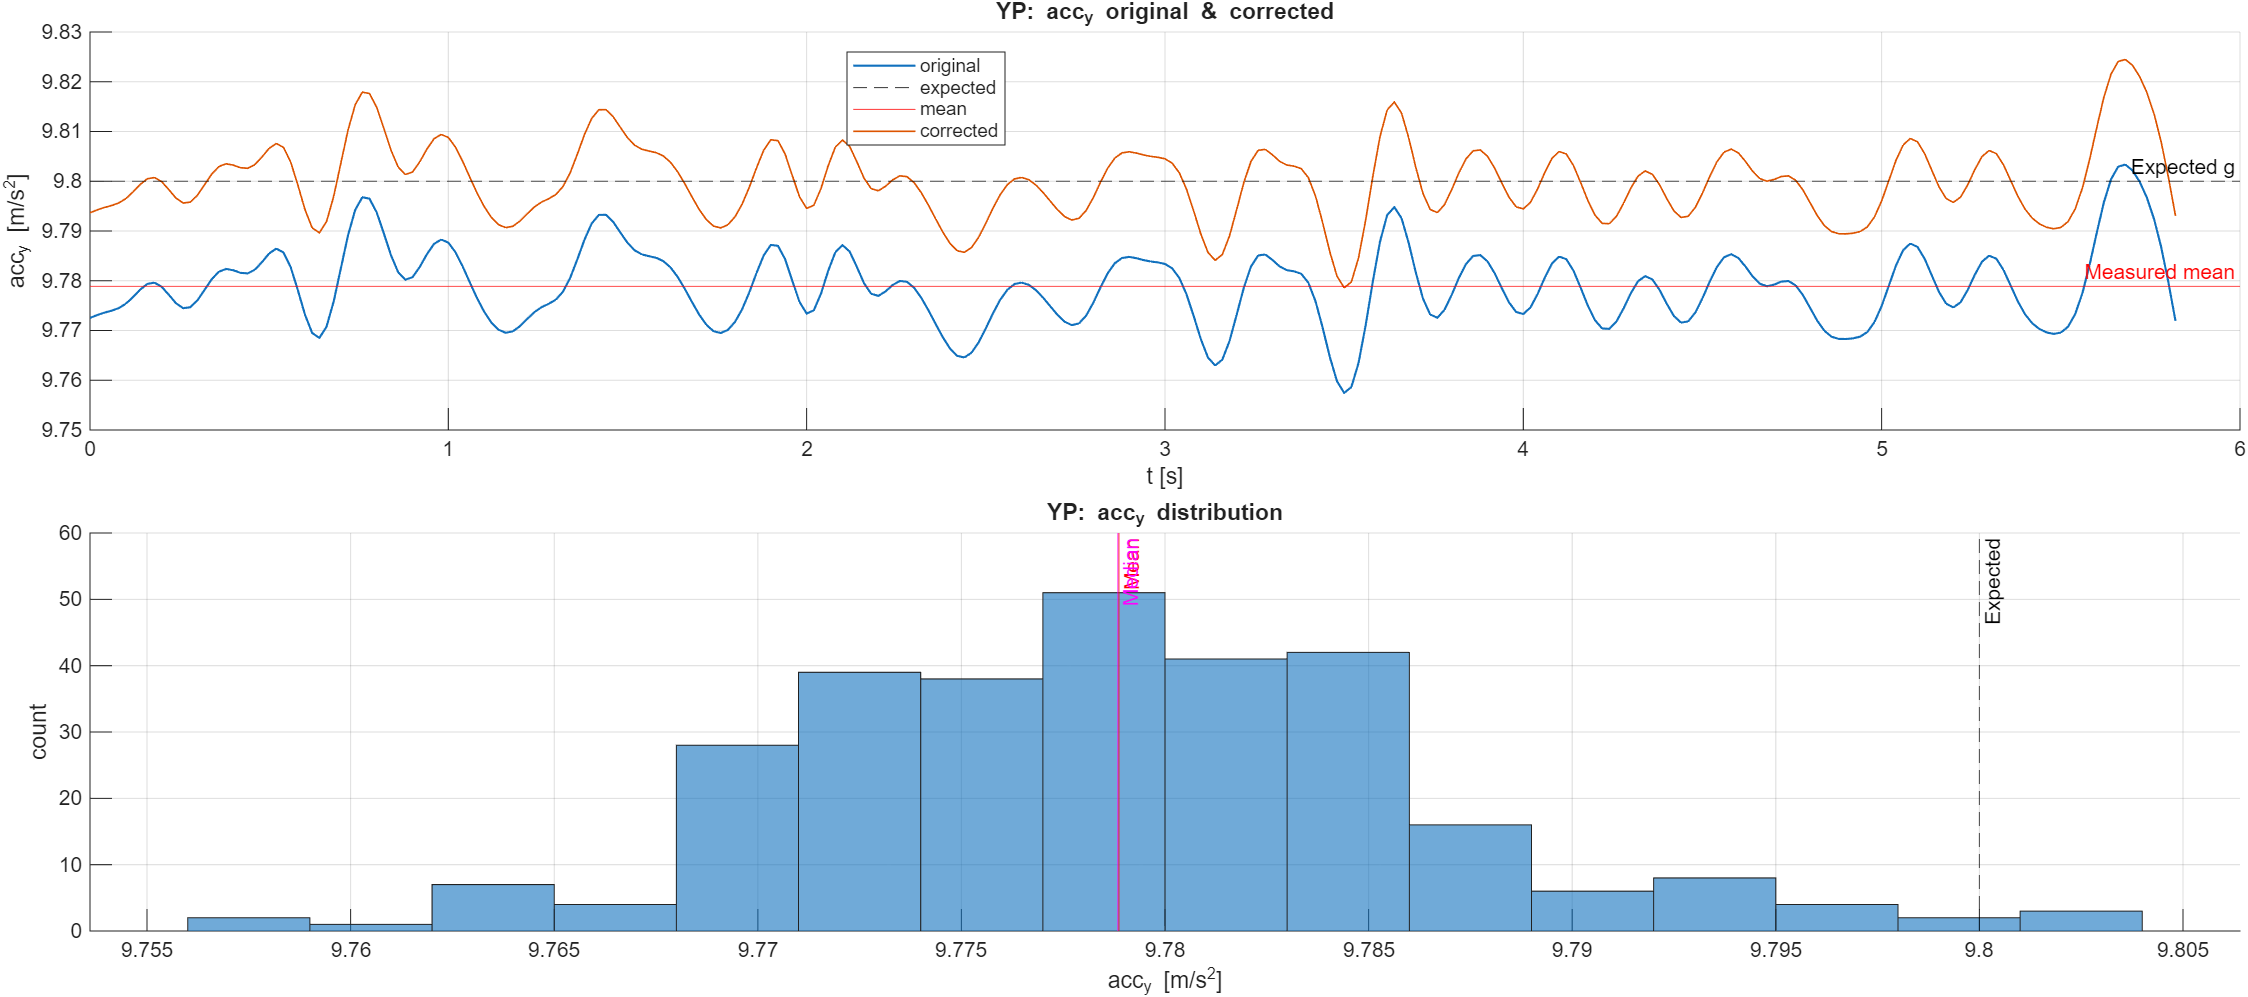
\includegraphics[width=0.3\columnwidth]{fig/Gravity check YP - acc_y.png}}
	\subcaptionbox{z positive
		\label{fig:calib_zp}}{
		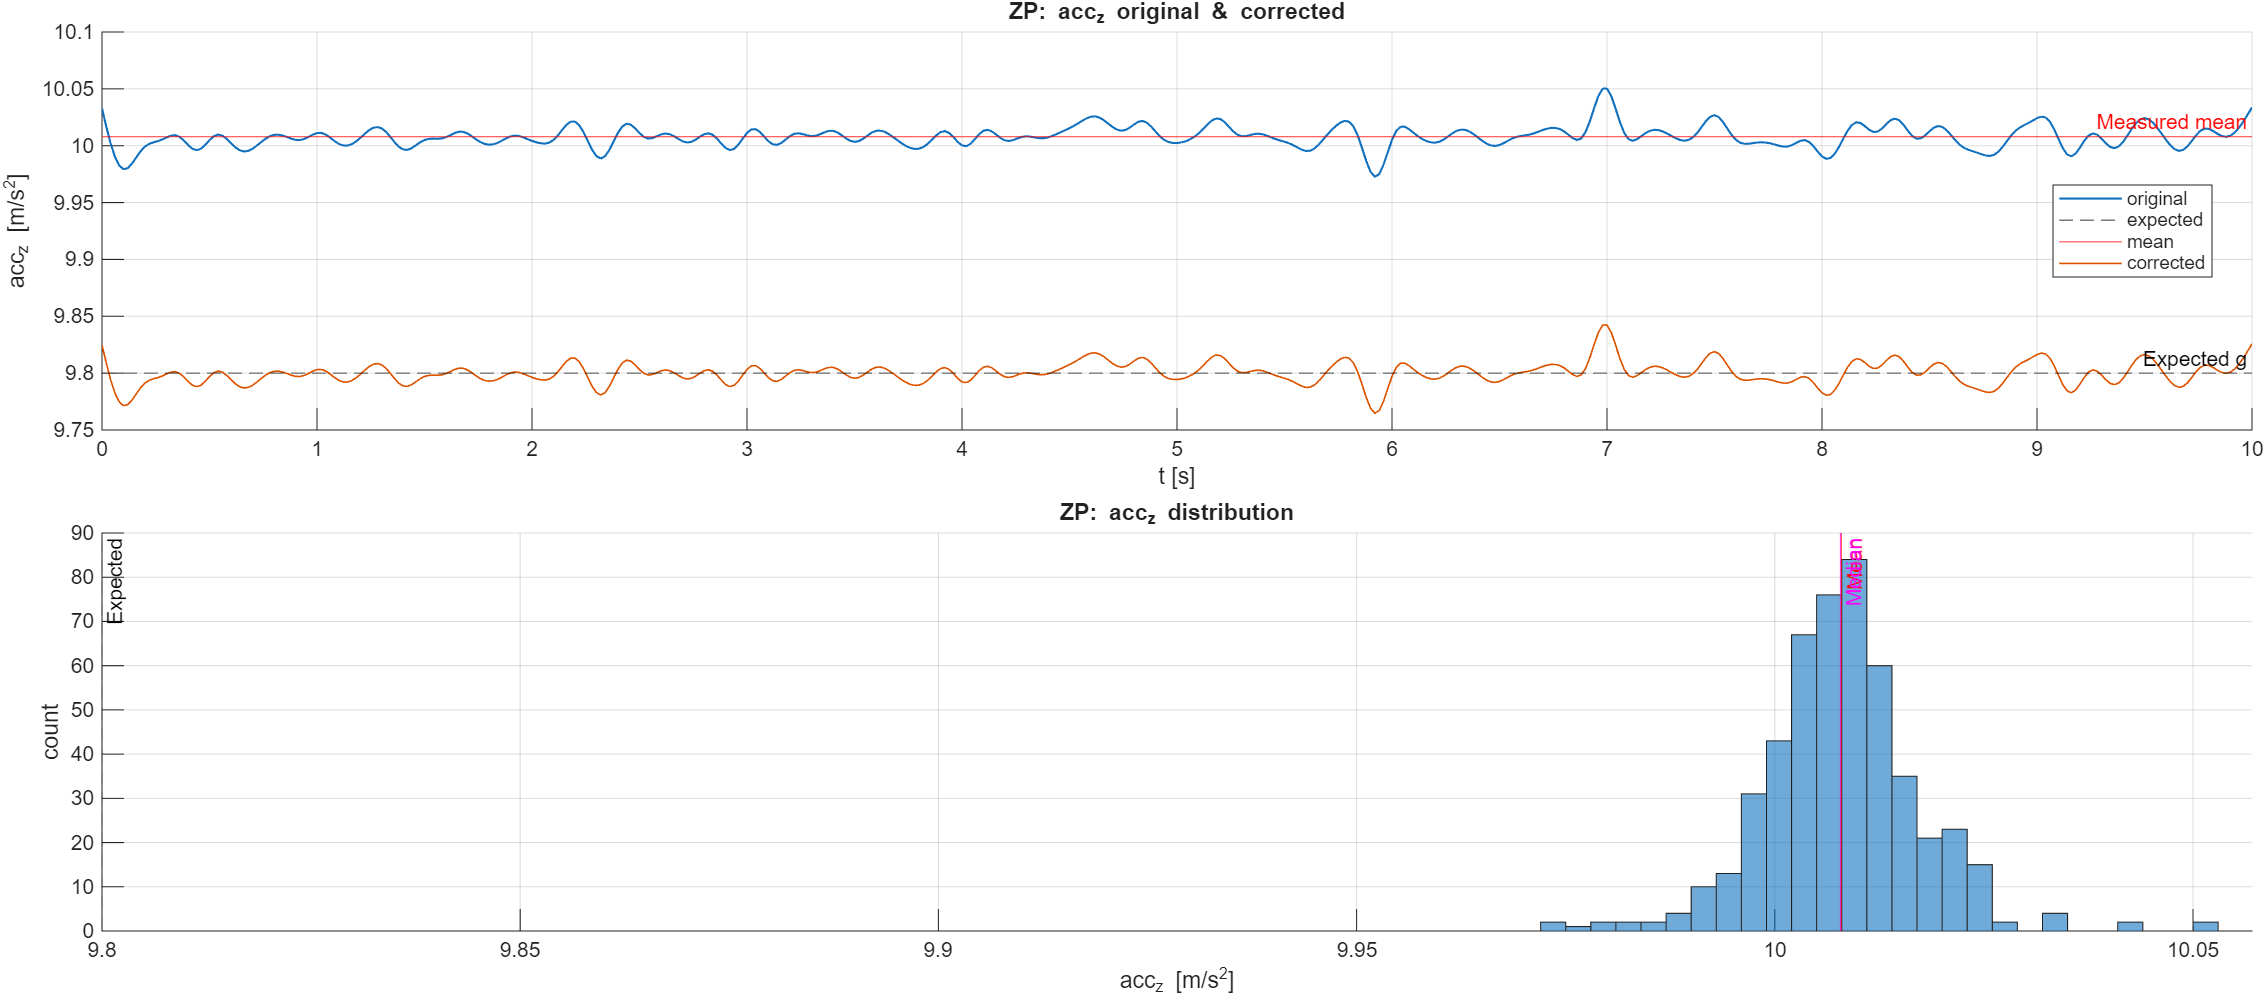
\includegraphics[width=0.3\columnwidth]{fig/Gravity check ZP - acc_z.png}}
    \\
	\subcaptionbox{x negative 
		\label{fig:calib_xn}}{
		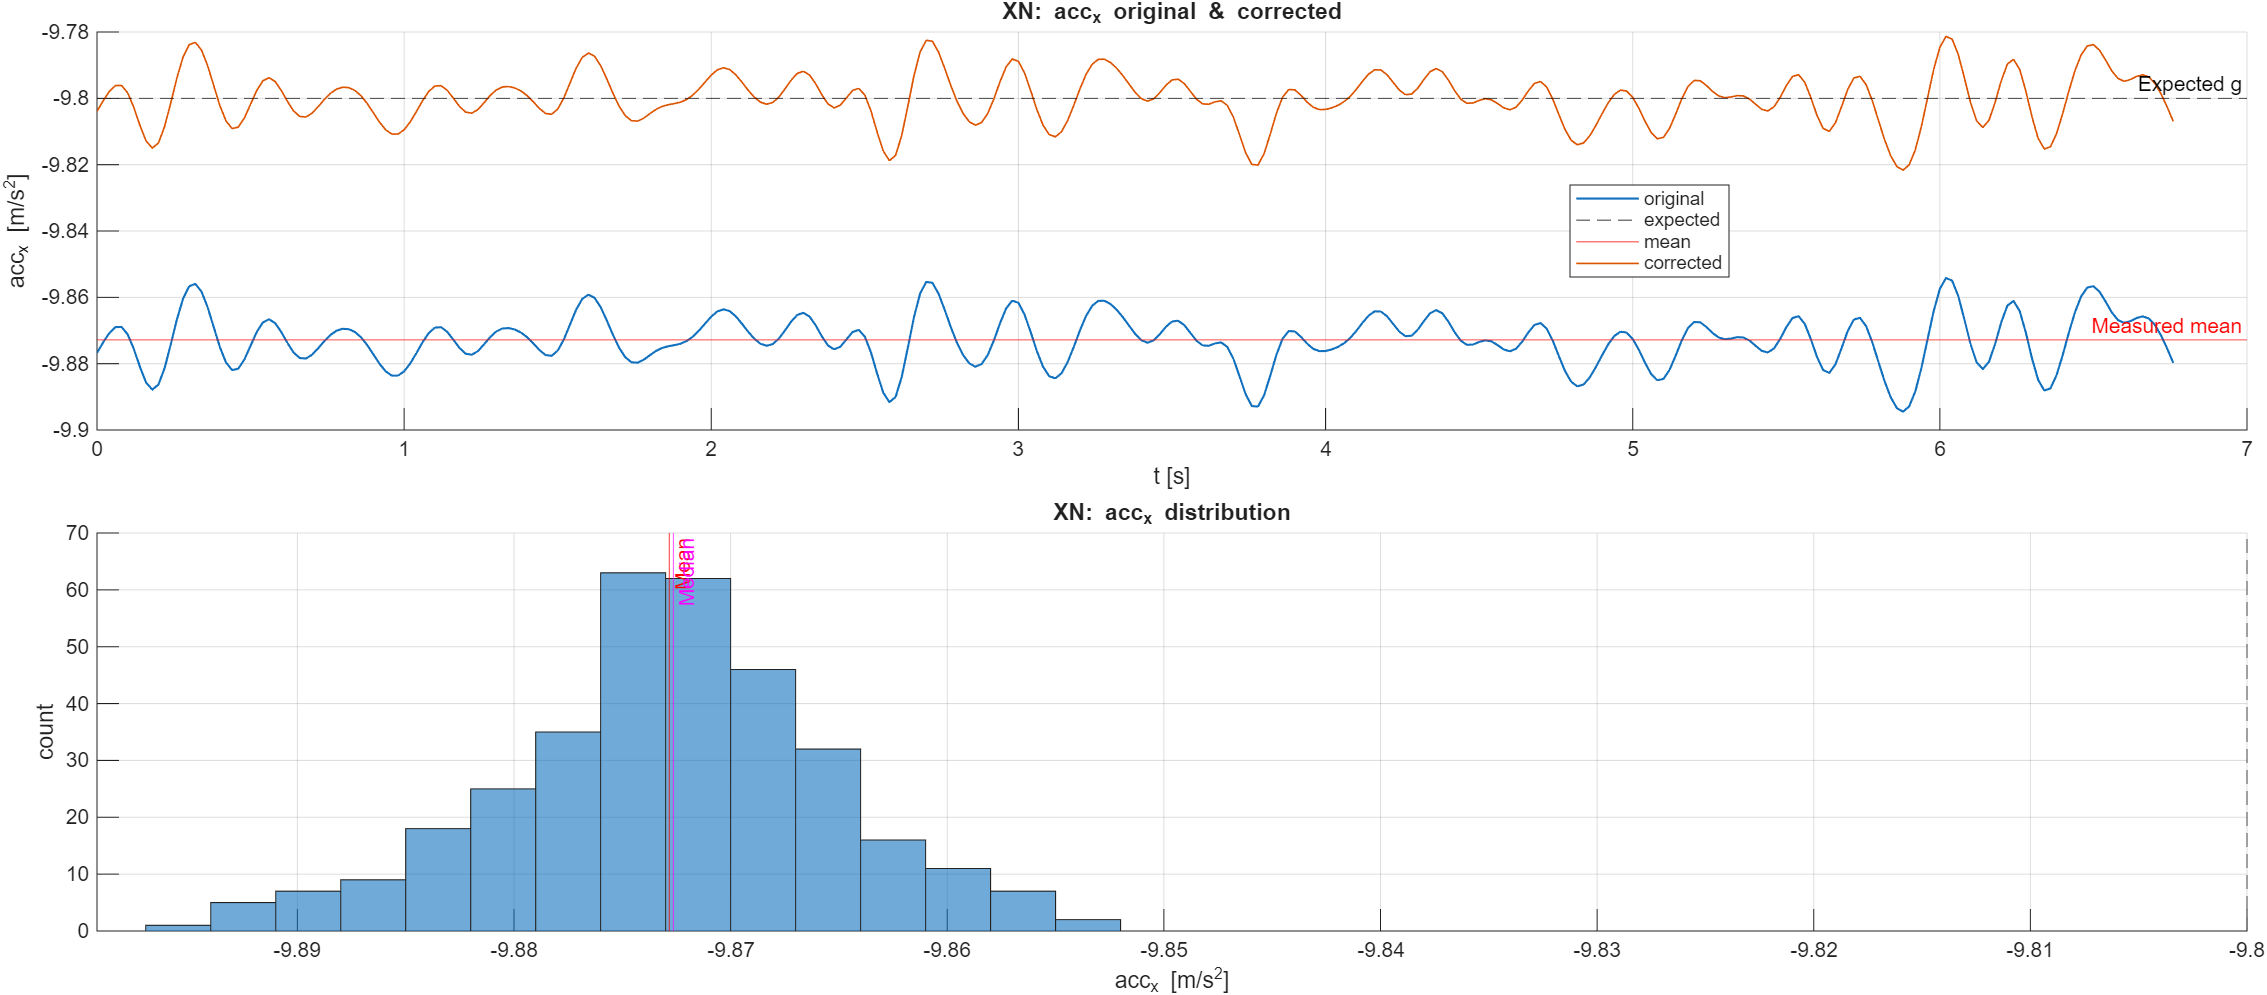
\includegraphics[width=0.3\columnwidth]{fig/Gravity check XN - acc_x.png}}
	\subcaptionbox{y negative 
		\label{fig:calib_yn}}{
		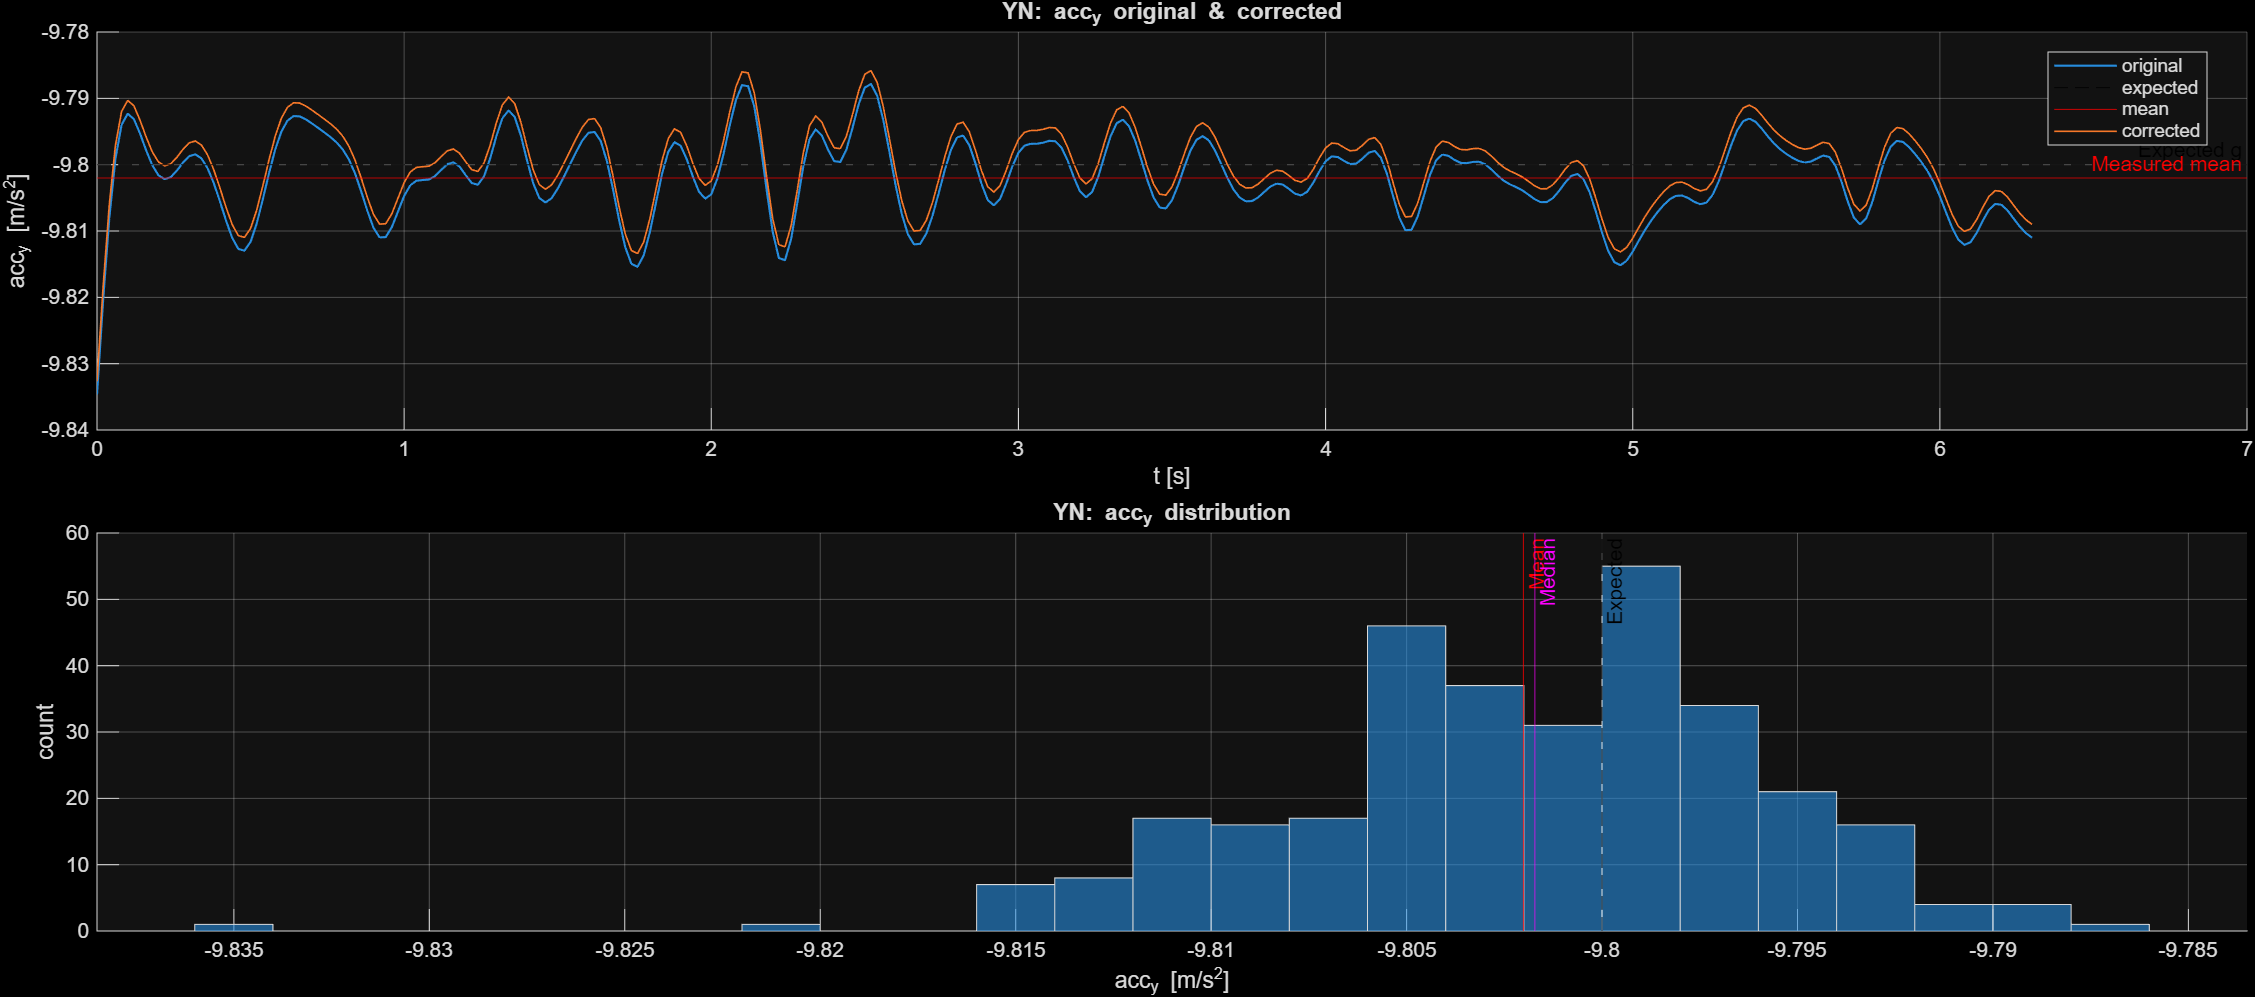
\includegraphics[width=0.3\columnwidth]{fig/Gravity check YN - acc_y.png}}
	\subcaptionbox{z negative 
		\label{fig:calib_zn}}{
		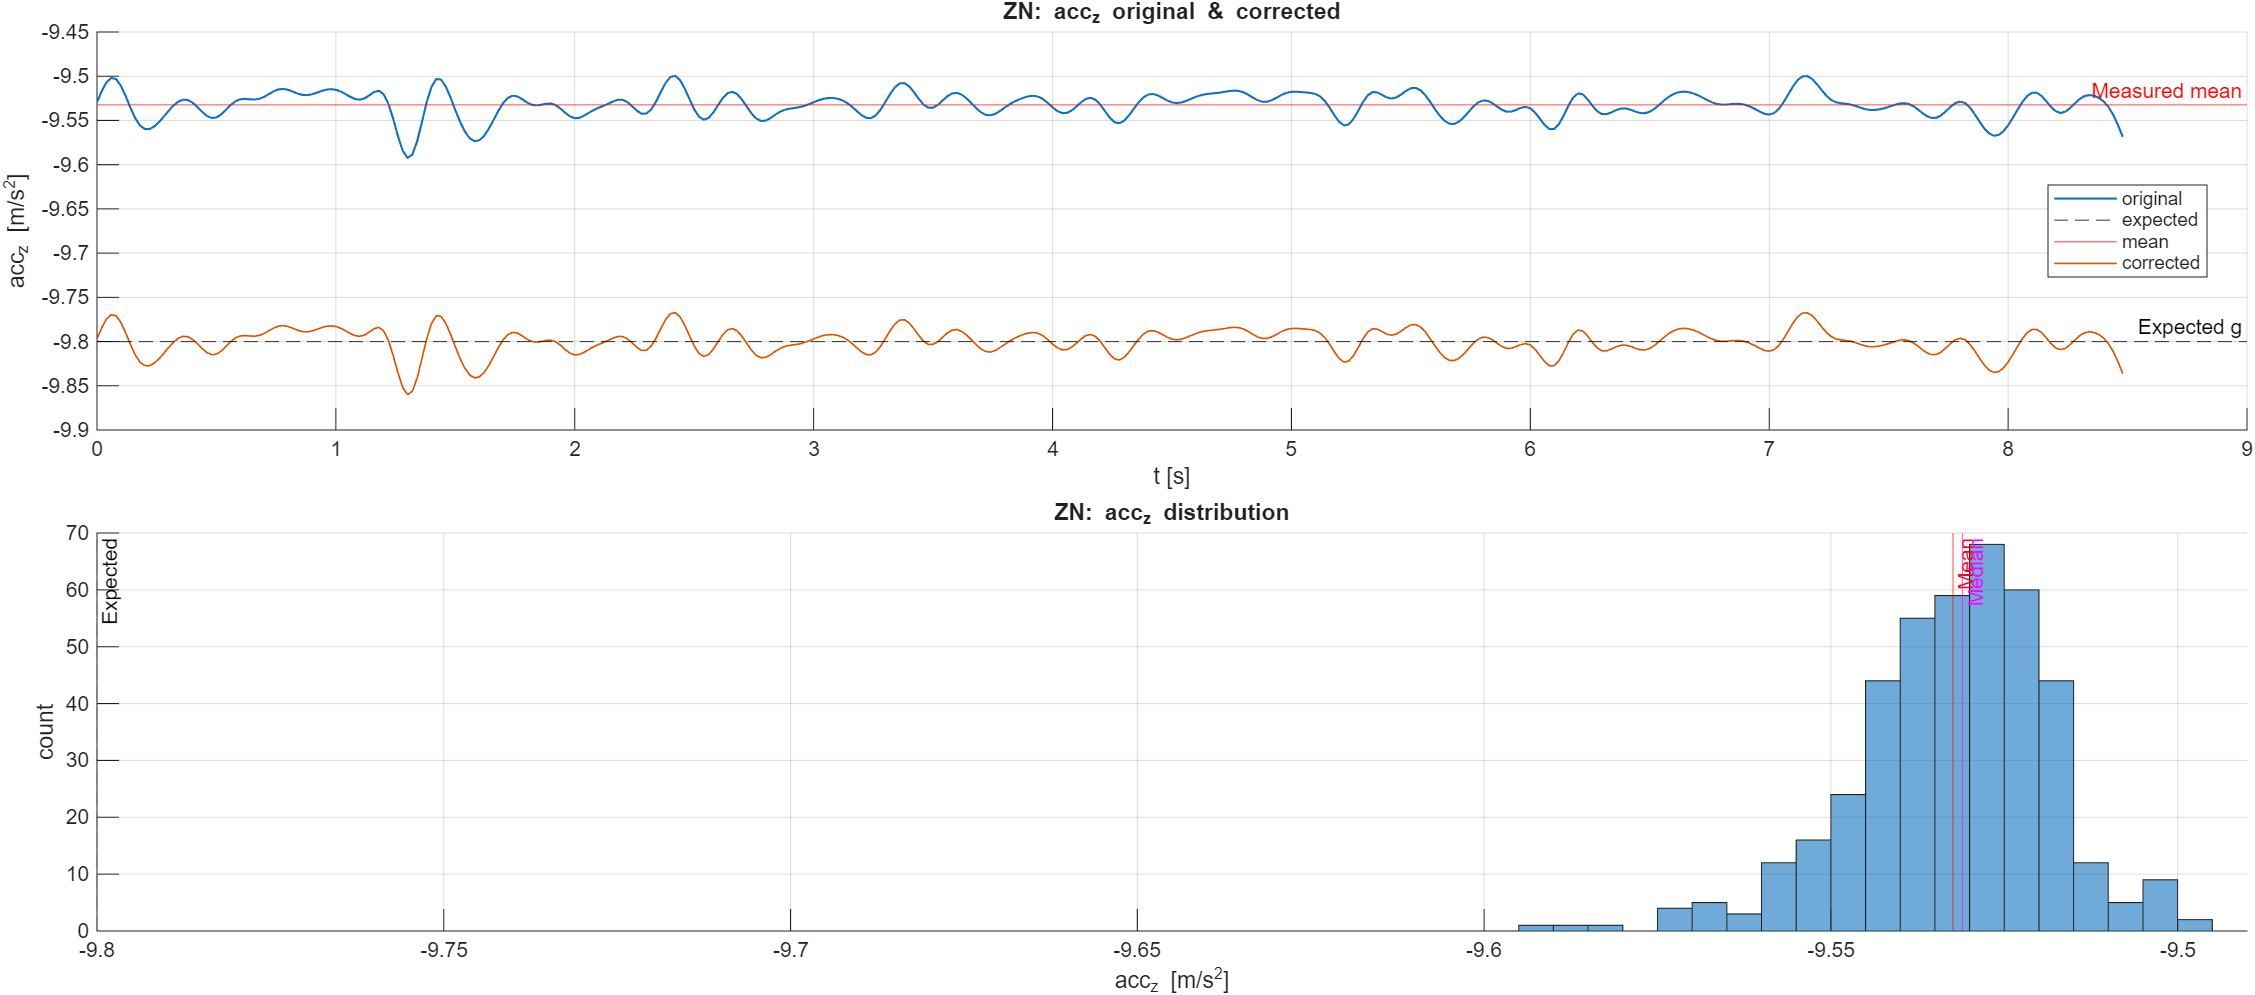
\includegraphics[width=0.3\columnwidth]{fig/Gravity check ZN - acc_z.png}}
	\caption{Calibration of accelleration on six different direction}
\label{fig:calibration_six}
\end{figure}

\subsection{Car Displacement}




\section{Experiment II: Walking Motion Detection}
\subsection{Calibration}
Since what we're interesting in is the total displacement on the three direction, in this section we directly pass the signal through a low pass filter.


\subsection{Coordinate System Transformation}
\subsection{Walking Motion Analysis}
\subsection{Walking Trace Reconstruction}



\pagebreak

\begin{thebibliography}{99}

\end{thebibliography}
\end{document}




